\documentclass[10pt,twocolumn,letterpaper]{article}
\usepackage{cvpr} % Use cvpr.sty for CVPR format
\usepackage{times}
\usepackage{epsfig}
\usepackage{graphicx}
\usepackage{amsmath}
\usepackage{amssymb}
\usepackage{graphicx}
\usepackage[hidelinks]{hyperref}
\usepackage{graphicx}
\usepackage{float}
\title{Convolutional Neural Networks for Image Classification}

\author{Shivangi \\
The University of Adelaide\\
Adelaide, South Australia, Australia\\
{\tt\small shivangi@student.adelaide.edu.au}
}
\begin{document}

\maketitle

\section{Abstract}
This report examines various Convolutional Neural Network (CNN) architectures—Basic CNN, ResNet-18, MobileNet, and AlexNet—on the CIFAR-10 dataset, focusing on data augmentation, hyperparameter tuning, and model-specific adaptations to optimize performance in resource-constrained environments. Each model was trained from scratch to evaluate its classification accuracy, computational efficiency, and generalization ability. ResNet-18 achieved the highest accuracy, while MobileNet demonstrated considerable efficiency in terms of computational resources, providing a suitable alternative for mobile or low-power applications. The findings support the use of lightweight architectures for efficient image classification in constrained settings.
\section{Introduction and Background}
Image classification is a fundamental task in computer vision with applications in various domains such as autonomous driving, medical diagnostics, and security. CIFAR-10, a standard dataset, consists of 60,000 32x32 images across 10 classes, serving as a benchmark for evaluating CNN models. This study implements and compares Basic CNN, ResNet-18, AlexNet, and MobileNet models to assess their performance on CIFAR-10 while balancing computational cost and accuracy.

ResNet-18's residual connections help manage gradient issues in deeper networks. AlexNet, a pioneering architecture, laid the foundation for deep learning's impact on classification tasks, while MobileNet's depthwise separable convolutions offer significant efficiency gains. This report aims to determine the optimal model for accurate and efficient classification in resource-constrained environments.
\section{Related Work}
CNNs revolutionized image classification, allowing for learning complex feature hierarchies directly from image data. ResNet’s architecture with residual connections effectively trains deep models by mitigating the vanishing gradient problem. AlexNet introduced dropout for regularization, achieving remarkable results on ImageNet. MobileNet, designed with depthwise separable convolutions, achieves high accuracy with fewer parameters, making it ideal for mobile devices and real-time applications.

Previous studies show that while ResNet generally outperforms in accuracy, lightweight models like MobileNet are faster and require fewer resources. This work extends the comparison to CIFAR-10, focusing on optimizing both resource efficiency and classification accuracy.
\section{Methodology}
\subsection{Dataset and Preprocessing}
CIFAR-10 contains 50,000 training images and 10,000 testing images across 10 classes. Each image was normalized to the range [0, 1] and data augmentation techniques such as random horizontal flips, rotations, and brightness adjustments were applied to enhance generalization. These transformations were applied probabilistically to diversify the training data and improve model robustness.
\begin{figure}[H]
    \centering
    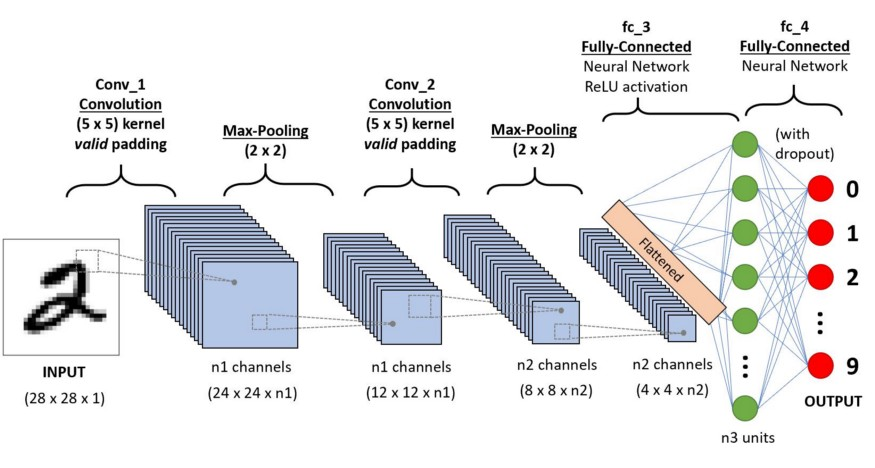
\includegraphics[width=0.5\textwidth]{D:/tri3/Deep Learning/Assignment-2/CNN_working.jpeg}
    \caption{Flowchart for Convolutional Neural Network}
    \label{fig1: Flowchart for Convolutional Neural Network}
\end{figure}
\begin{figure}[H]
    \centering
    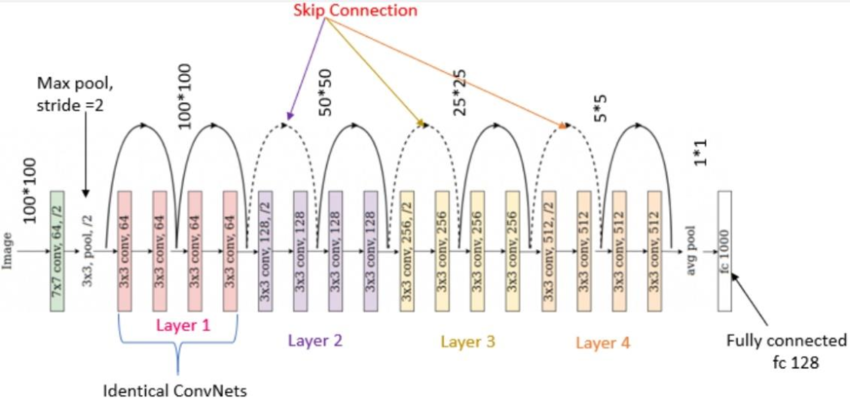
\includegraphics[width=0.5\textwidth]{D:/tri3/Deep Learning/Assignment-2/ResNet-18.png}
    \caption{Flowchart for Convolutional Neural Network}
    \label{fig1: Implementation of ResNet-18}
\end{figure}
\begin{figure}[H]
    \centering
    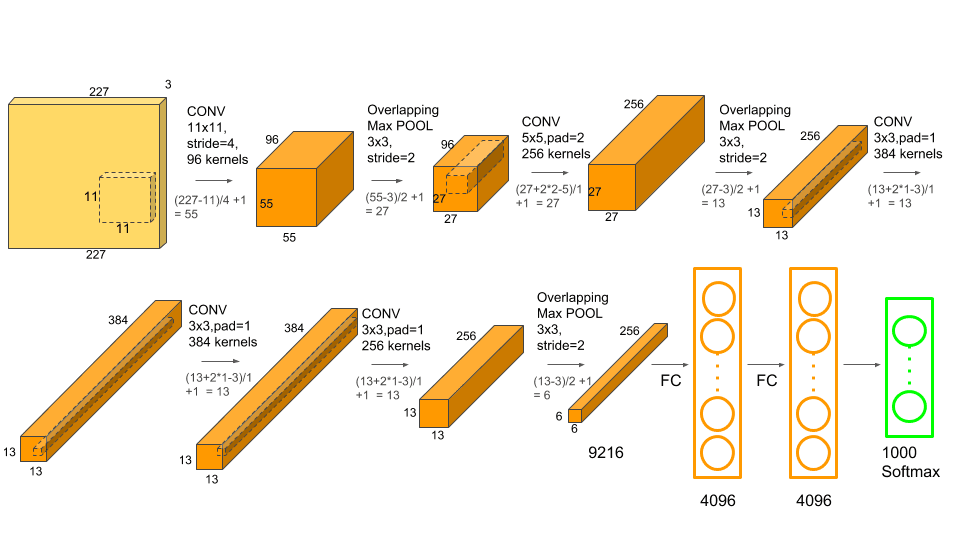
\includegraphics[width=0.5\textwidth]{D:/tri3/Deep Learning/Assignment-2/Alexnet.png}
    \caption{Flowchart for Convolutional Neural Network}
    \label{fig1: Implementation of AlexNet}
\end{figure}
\begin{figure}[H]
    \centering
    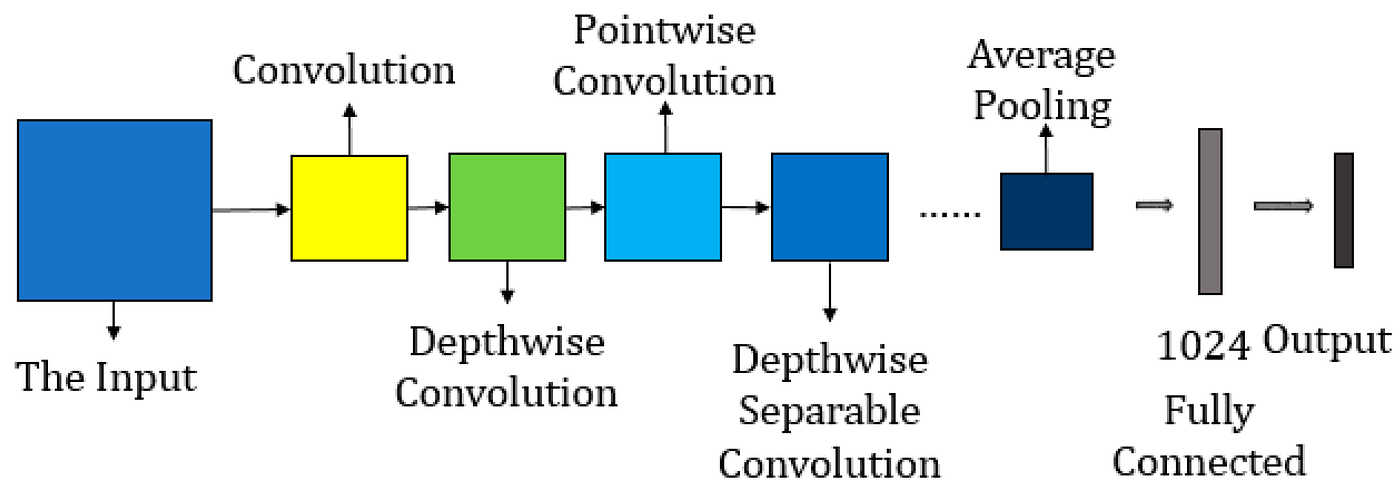
\includegraphics[width=0.5\textwidth]{D:/tri3/Deep Learning/Assignment-2/Mobilenet.png}
    \caption{Flowchart for Convolutional Neural Network}
    \label{fig1: Implementation of MobileNet}
\end{figure}
\subsection{Model Architecture}
\subsubsection{Basic CNN Model}: This model was constructed as a simple convolutional network with multiple convolutional and pooling layers followed by fully connected layers. It serves as a baseline to compare more advanced architectures. The model includes ReLU activations and max-pooling layers to downsample feature maps, extracting meaningful spatial information while reducing computational load as shown in figure-1.

\subsubsection{ResNet-18} As from the figure-2 it can be seen that The ResNet-18 architecture is composed of 18 layers , organized in residual blocks, where each block contains shortcut connections to bypass certain layers. This configuration addresses the vanishing gradient problem and allows the network to maintain performance as it grows deeper. Residual blocks ensure that the model can learn identity mappings if needed, aiding in stable convergence (He et al., 2016).

\subsubsection{AlexNet} Originally designed for high-dimensional image data, AlexNet consists of convolutional and fully connected layers, with ReLU activations and max-pooling layers following each convolution. The architecture uses dropout regularization in its dense layers to mitigate overfitting, making it a relevant choice for CIFAR-10, albeit simplified for our use (Krizhevsky et al., 2012).The architechture of the same is shown in figure3.

\subsubsection{MobileNet} This lightweight architecture uses depthwise separable convolutions to reduce the number of parameters and computational requirements while maintaining competitive accuracy. MobileNet is particularly suited for real-time and mobile applications (Howard et al., 2017). It leverages both depthwise and pointwise convolutions to build feature representations efficiently, making it ideal for deployment on hardware with limited resources.The architechture of the same is shown in figure4.


\subsection{Training Setup and Hyperparameter Tuning}
All models were trained using the Adam optimizer with an initial learning rate of 0.001 and a batch size of 32. Early stopping based on validation loss was applied to prevent overfitting. Grid search was employed to tune hyperparameters, focusing on:

\subsubsection{Learning Rate} Adjustments were made to ensure stable convergence.
\subsubsection{Optimizer:}Adam was selected for its adaptive learning capabilities.
\subsubsection{Regularization:} Dropout was implemented in AlexNet and Basic CNN to mitigate overfitting. Trials with and without residual links in ResNet-18 were conducted to assess their impact on performance.
\section{Experiment Design}
Experiments were conducted under consistent conditions to evaluate model performance. Key objectives included:

\subsubsection{Comparing Architectures}  Analyze the effectiveness of each model—Basic CNN, ResNet-18, AlexNet, and MobileNet—on CIFAR-10.
\subsubsection{Hyperparameter Tuning} Assess the effects of different learning rates, dropout rates, and data augmentation.
\subsubsection{Residual Connections}Measure the impact of residual blocks in ResNet-18 on convergence and accuracy.
\section{Result}
Figures below present the training and validation accuracy/loss for each model, demonstrating the results for hyperparameter tuning and model comparisons.

\subsubsection{ResNet-18} Achieved the highest accuracy with stable convergence, supported by residual connections.Figure 4 and 5 shows training and validation accuracy/loss for ResNet-18

\begin{figure}[H]
    \centering
    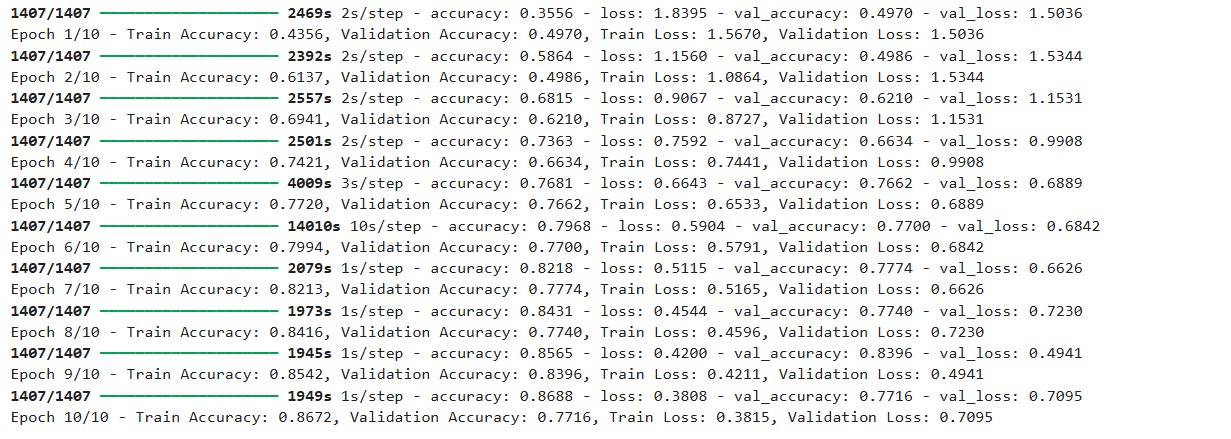
\includegraphics[width=0.5\textwidth]{D:/tri3/Deep Learning/Assignment-2/resnet-18_Acc.png}
    \caption{Training and validation accuracy/loss for ResNet-18}
    \label{fig1: Implementation of AlexNet}
\end{figure}
\subsubsection{AlexNet and MobileNet} Showed balanced performance, with MobileNet achieving competitive accuracy with significantly lower resource usage. shown in figure 6 and 7.

\begin{figure}[H]
    \centering
    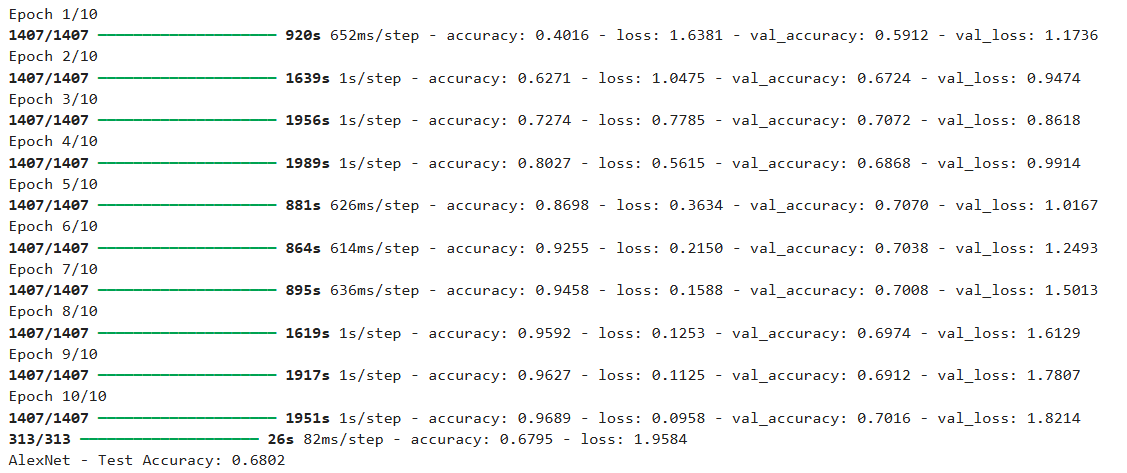
\includegraphics[width=0.5\textwidth]{D:/tri3/Deep Learning/Assignment-2/alexnet_acc.png}
    \caption{Training and validation Accuracy/Loss for AlexNet }
    \label{fig1: Implementation of AlexNet}
\end{figure}
\begin{figure}[H]
    \centering
    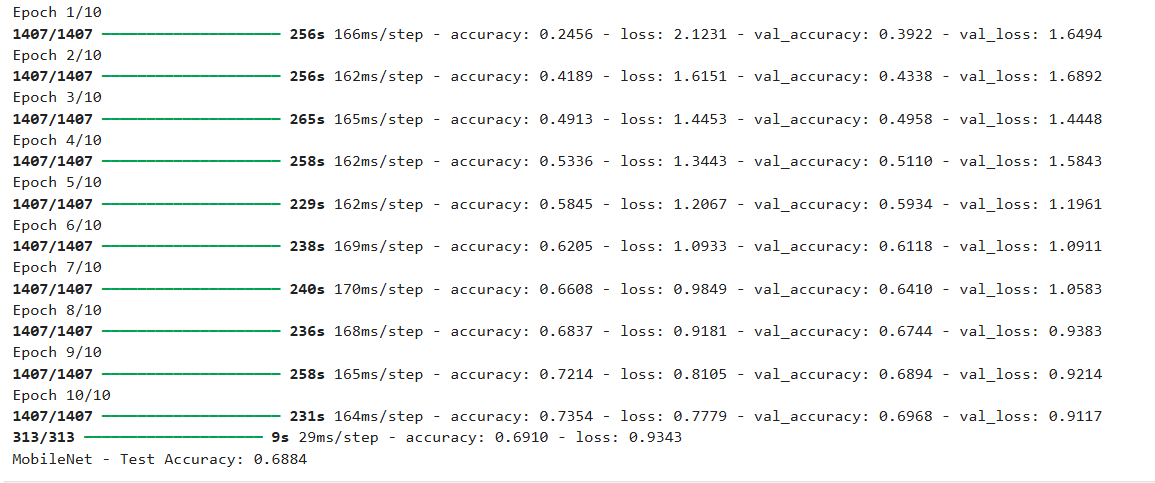
\includegraphics[width=0.5\textwidth]{D:/tri3/Deep Learning/Assignment-2/mobilenet_acc.png}
    \caption{Training and validation Accuracy/Loss for MobileNet }
    \label{fig1: Implementation of AlexNet}
\end{figure}
\subsubsection{Basic CNN} As expected, performed modestly compared to advanced models but provided a strong baseline. Include visual results here: 

\begin{figure}[H]
    \centering
    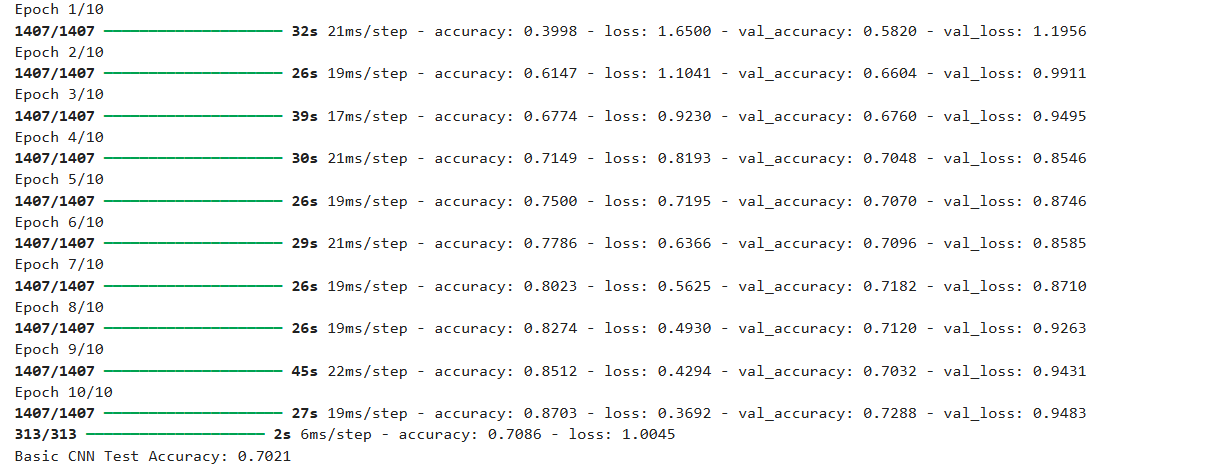
\includegraphics[width=0.5\textwidth]{D:/tri3/Deep Learning/Assignment-2/basic_cnn_acc.png}
    \caption{Training and validation Accuracy/Loss for CNN }
    \label{fig1: Implementation of AlexNet}
\end{figure}

\subsubsection{Training and validation Accuracy/Loss for Models at different learning rate andoptimizer adam}
Test Accuracy for LR 0.0001 with optimizer adam: 0.7285
\begin{figure}[H]
    \centering
    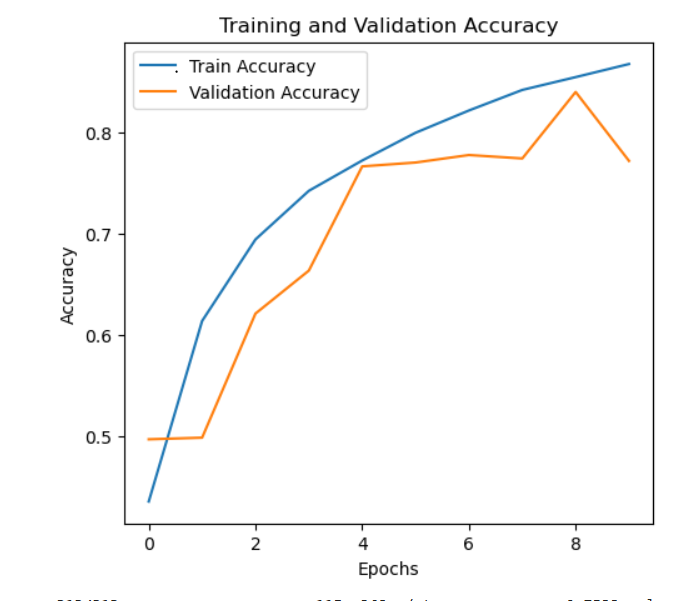
\includegraphics[width=0.5\textwidth]{D:/tri3/Deep Learning/Assignment-2/Restnet_plot_accl.png}
    \caption{Training and validation accuracy for ResNet-18}
    \label{fig1: Implementation of AlexNet}
\end{figure}
\begin{figure}[H]
    \centering
    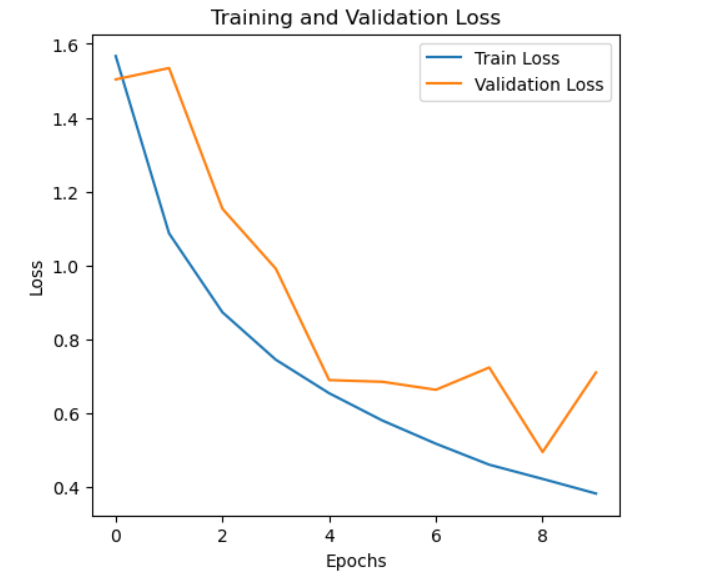
\includegraphics[width=0.5\textwidth]{D:/tri3/Deep Learning/Assignment-2/Restnet_plot_loss.png}
    \caption{Training and validation Loss for ResNet-18}
    \label{fig1: Implementation of AlexNet}
\end{figure}

Test Accuracy for LR 0.0001 with optimizer SGD: 0.7261

\begin{figure}[H]
    \centering
    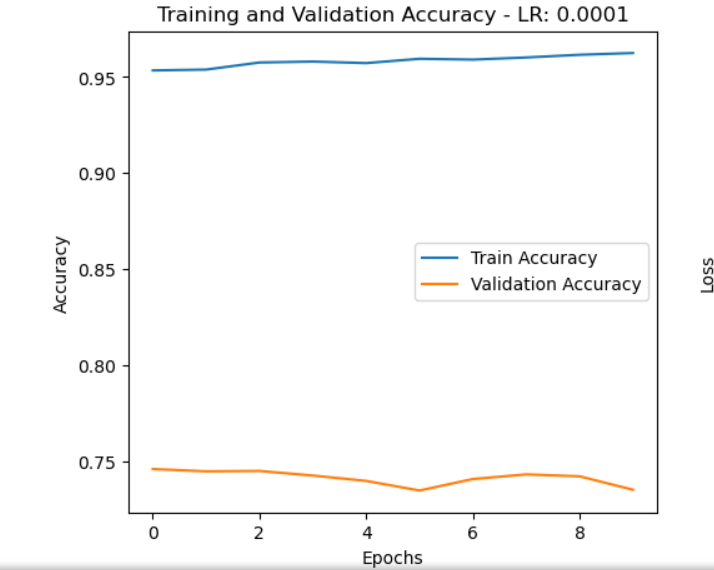
\includegraphics[width=0.5\textwidth]{D:/tri3/Deep Learning/Assignment-2/diffl.png}
    \caption{Training and validation Accuracy }
    \label{fig1: Implementation of AlexNet}
\end{figure}
\begin{figure}[H]
    \centering
    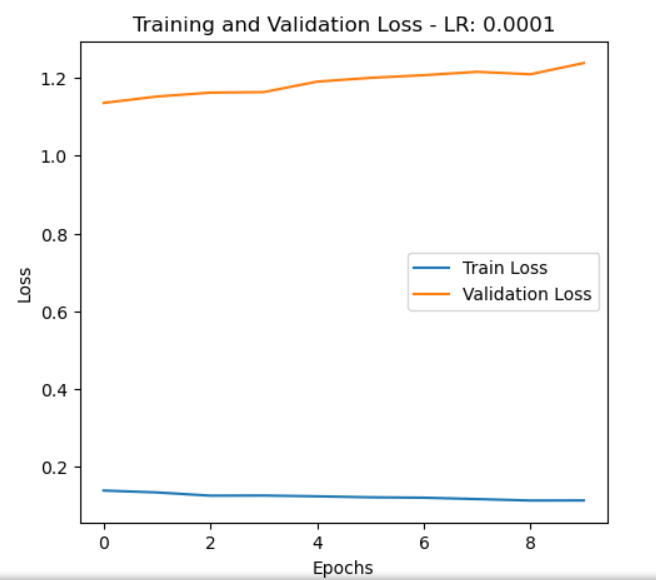
\includegraphics[width=0.5\textwidth]{D:/tri3/Deep Learning/Assignment-2/diffac.png}
    \caption{Training and validation loss }
    \label{fig1: Implementation of AlexNet}
\end{figure}
Test Accuracy for LR 0.001 with optimizer adam: 0.7138
\begin{figure}[H]
    \centering
    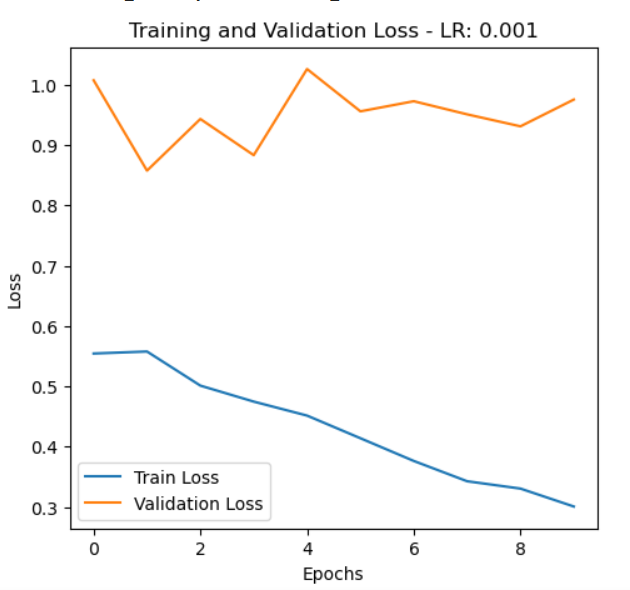
\includegraphics[width=0.5\textwidth]{D:/tri3/Deep Learning/Assignment-2/loss07.png}
    \caption{Training and validation loss}
    \label{fig1: Implementation of AlexNet}
\end{figure}
\begin{figure}[H]
    \centering
    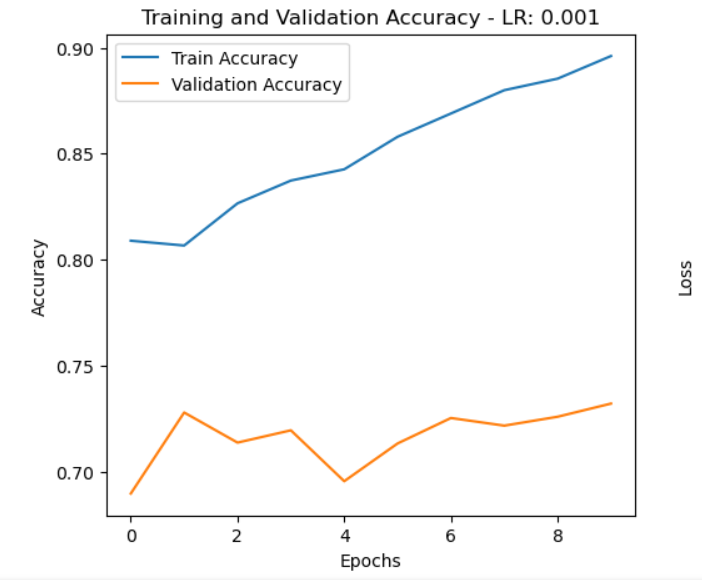
\includegraphics[width=0.5\textwidth]{D:/tri3/Deep Learning/Assignment-2/acc07.png}
    \caption{Training and validation Accuracy }
    \label{fig1: Implementation of AlexNet}
\end{figure}
\section{Discussion}
The results indicate that ResNet-18 is well-suited for accuracy-focused applications, achieving the highest classification accuracy on CIFAR-10. Residual connections allowed it to maintain stability during training, which is beneficial for deeper networks. MobileNet, on the other hand, demonstrated strong performance with fewer computational resources, making it ideal for real-time and mobile applications.

The analysis of learning rates revealed that all models required tuning to achieve optimal performance. AlexNet benefited from dropout regularization, which mitigated overfitting, while the Basic CNN model offered baseline insights into the benefits of more advanced architectures.
\section{Conclusion and Future Work}This study explored Basic CNN, ResNet-18, AlexNet, and MobileNet for CIFAR-10 image classification, identifying ResNet-18 as the best performer in terms of accuracy and MobileNet as the most efficient for resource-constrained environments. The findings underscore the significance of lightweight architectures and effective hyperparameter tuning for practical applications in constrained environments.

Future work could expand on these findings by exploring other lightweight models, advanced regularization techniques, and pre-trained models on more complex datasets. These approaches could further enhance the accuracy and efficiency of CNN models for real-world applications.
\section{Code}
My code and data is available GitHub: \href{ https://github.com/shivangi-crypto/CNN_Image_classification.git}{CNN Image Classification}.
\section{References}
1.He, K., Zhang, X., Ren, S., and Sun, J., 2016.  Deep residual learning for image recognition. In Proceedings of the IEEE conference on computer vision and pattern recognition (pp. 770-778).
2.Howard, A.G., Zhu, M., Chen, B., et al., 2017. MobileNets: Efficient convolutional neural networks for mobile vision applications. arXiv preprint arXiv:1704.04861.
3.Krizhevsky, A., Nair, V., and Hinton, G., 2009. Learning multiple layers of features from tiny images. University of Toronto.
4.Krizhevsky, A., Sutskever, I., and Hinton, G.E., 2012. ImageNet classification with deep convolutional neural networks. Advances in Neural Information Processing Systems, 25.
\end{document}